
%(BEGIN_QUESTION)
% Copyright 2006, Tony R. Kuphaldt, released under the Creative Commons Attribution License (v 1.0)
% This means you may do almost anything with this work of mine, so long as you give me proper credit

Her vises en destillasjonskolonne, brukt til å separere en væskeblanding av stoffer i de enkelte komponentene. Prosessen med {\it destillasjon}, eller {\it fraksjonering} som den også kalles, er svært vanlig i tung prosessindustri, spesielt i petrokjemisk prosessering:

$$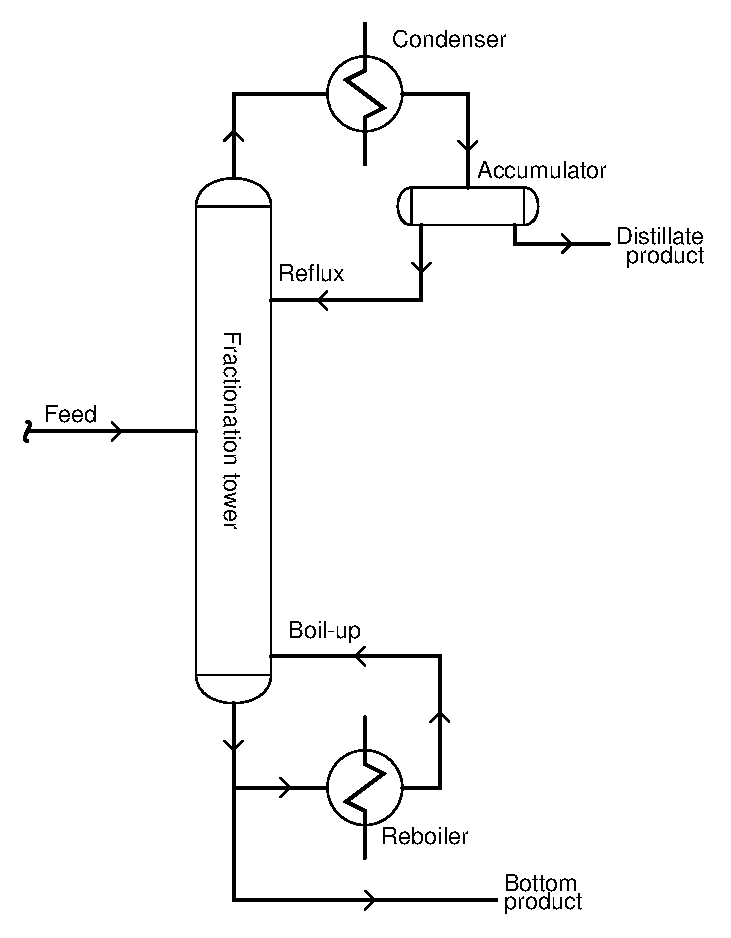
\includegraphics[width=15.5cm]{i01376x01.eps}$$

De lette dampene som tas ut fra toppen av en destillasjonskolonne kondenseres på nytt i en ``akkumulator'' og føres tilbake til fraksjoneringsprosessen som ``refluks''. De tunge dampene som kondenserer i bunnen av kolonnen kokes opp igjen til dampform og føres tilbake til fraksjoneringsprosessen som ``boil-up''. Det er nødvendig å føre refluks og boil-up tilbake i kolonnen for å rense sluttproduktene mest mulig. P\&ID-en som vises her er uten instrumentering for enkelhets skyld.

\filbreak

Her er en enkel refluks-reguleringssløyfe vist, for å regulere mengden refluks som føres inn i kolonnen fra akkumulatoren:

$$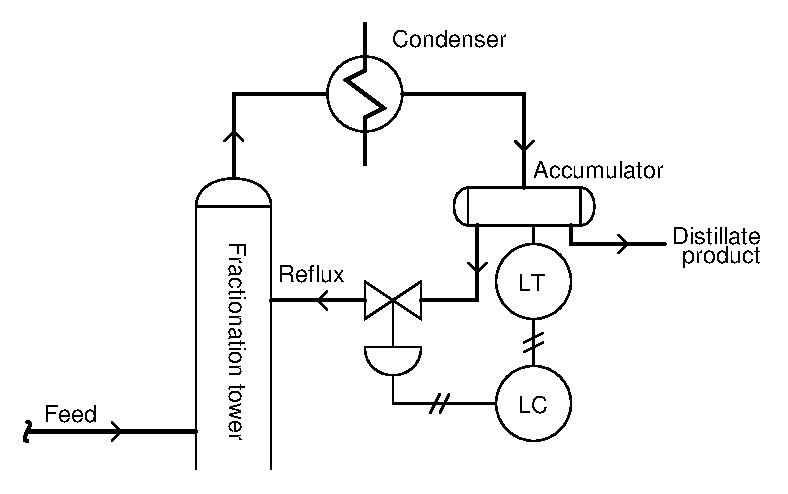
\includegraphics[width=15.5cm]{i01376x02.eps}$$

Kolonnen drives med regulert trykk på 75 PSI. Refluks strømmer fra akkumulatoren, gjennom ventilen og inn i kolonnen kun ved hjelp av gravitasjon. Høydeforskjellen mellom akkumulatorens konstante væskenivå og refluks-reguleringsventilen er 12 fot, og refluksproduktet er flytende pentan (spesifikk vekt = 0.6262). Hvis ønsket maksimal refluksrate gjennom ventilen er 500 GPM, hva må da ventilens $C_v$ være?

\vskip 20pt \vbox{\hrule \hbox{\strut \vrule{} {\bf Forslag til sokratisk diskusjon} \vrule} \hrule}

\begin{itemize}
\item{} Nevn noen praktiske formål for destillasjonskolonner i industrien.
\item{} Hvilken av de to varmevekslerne {\it tilfører} varme til kolonnen?
\item{} Hvilken av de to varmevekslerne {\it fjerner} varme fra kolonnen?
\item{} Anta at væsken i akkumulatoren var noe annet enn pentan (dvs. spesifikk vekt ikke var 0.6262). Hvordan ville dette påvirke dimensjoneringen av reguleringsventilen, dersom samme maksimale strømningsrate på 500 GPM fortsatt var ønsket?
\item{} Identifiser virkningene av at LT feiler med høyt signal (100\% væskenivå) i dette reguleringssystemet.
\item{} Identifiser virkningene av at LC blir stående i manuell modus uten oppfølging i dette reguleringssystemet.
\end{itemize}

\underbar{file i01376}
%(END_QUESTION)





%(BEGIN_ANSWER)

$C_v$ = 219.22

%(END_ANSWER)





%(BEGIN_NOTES)

$$\Delta P = \left(12 \hbox{ ft pentane} \over 1 \right)  \left(12 \hbox{ in} \over 1 \hbox{ ft}\right)  \left(1 \hbox{ PSI} \over 27.68 \hbox{ "WC}\right)  \left(0.6262 \hbox{ "WC} \over 1 \hbox{ "pentane}\right) = 3.258 \hbox{ PSID}$$

$$Q = C_v \sqrt{\Delta P \over G_f}$$

$$C_v = {Q \over \sqrt{\Delta P \over G_f}}$$

$$C_v = {500 \over \sqrt{3.258 \over 0.6262}} = 219.22$$

\vskip 10pt

Merk at ventilens $\Delta P$ utelukkende genereres av nivåhøyden mellom akkumulatorens væskenivå og reguleringsventilen. Kolonnetrykket på 75 PSI er irrelevant for beregning av ventilens kapasitetskoeffisient.

Interessant nok er væskens tetthet heller ikke relevant i akkurat dette tilfellet, siden gravitasjon er den eneste kraften som driver strømmen gjennom ventilen. Et enkelt tankeeksperiment bekrefter dette: prøv å doble spesifikk vekt og se hva som skjer. Hvis $G_f$ dobles, dobles også differansetrykket over ventilen som følge av 12 fot nivåhøyde. Men det samme gjør tetthetsleddet i ventilens $C_v$-formel, slik at verdien av brøken inne i radikanden ($\Delta P \over G_f$) forblir konstant uavhengig av væskens tetthet.

%INDEX% Final Control Elements, valve: sizing
%INDEX% Process: distillation (pentane)

%(END_NOTES)

